\documentclass[11pt]{article}
\usepackage[margin=1in]{geometry}
\usepackage{graphicx}
\usepackage{booktabs}
\usepackage{array}
\usepackage{xurl}
\usepackage{caption}
\usepackage{amsmath}
\captionsetup{font=small,labelfont=bf}
\setlength{\parindent}{0pt}
\setlength{\parskip}{6pt}
\emergencystretch=2em

\begin{document}

\begin{center}
{\Large Supplementary Information}\\[6pt]
{\large Auditing observability bias in InSAR-derived subsidence exposure estimates with a reproducible geospatial workflow}
\end{center}

This Supplementary Information provides reviewer-facing robustness and traceability material for the main manuscript. The figures and table support the same bounded claim as the main text: weakly observed exposure is retained for audit, not interpreted as confirmed damage or dense site-level validation.

\section*{Supplementary Figures}

\begin{figure}[htbp]
  \centering
  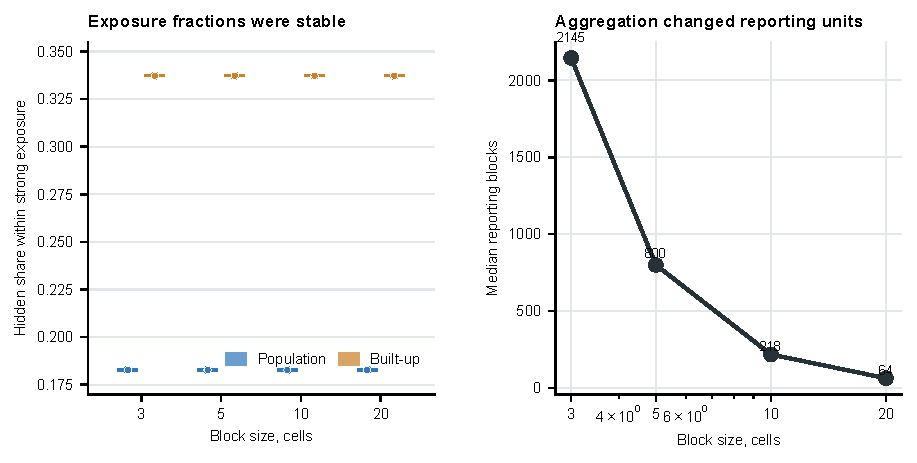
\includegraphics[width=0.98\linewidth]{ESIN_Supplementary_Figure_S1.pdf}
  \caption{MAUP and shifted-origin sensitivity. The left panel shows that hidden population and built-up shares within the strong-exposure layer remained stable across tested block sizes and shifted origins. The right panel shows that the reporting units changed substantially as block size increased. The result supports the interpretation that the retained hidden exposure is not an artefact of one reporting partition.}
  \label{fig:S1}
\end{figure}

\begin{figure}[htbp]
  \centering
  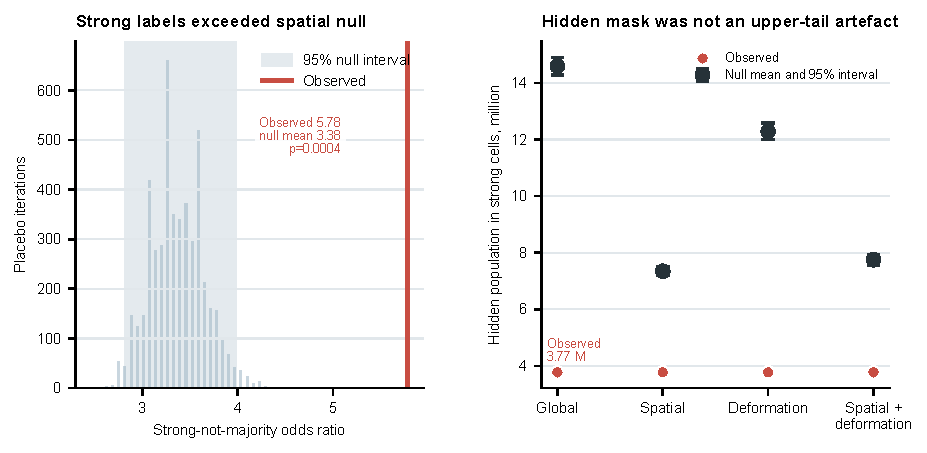
\includegraphics[width=0.98\linewidth]{ESIN_Supplementary_Figure_S2.pdf}
  \caption{Placebo randomization checks. The left panel compares the observed strong-not-majority-observable odds ratio with the spatial placebo null distribution. The right panel compares the observed hidden population in strong cells with null expectations from random hidden-mask models. The checks are falsification tests for random label or mask placement and are not interpreted as independent deformation validation.}
  \label{fig:S2}
\end{figure}

\begin{figure}[htbp]
  \centering
  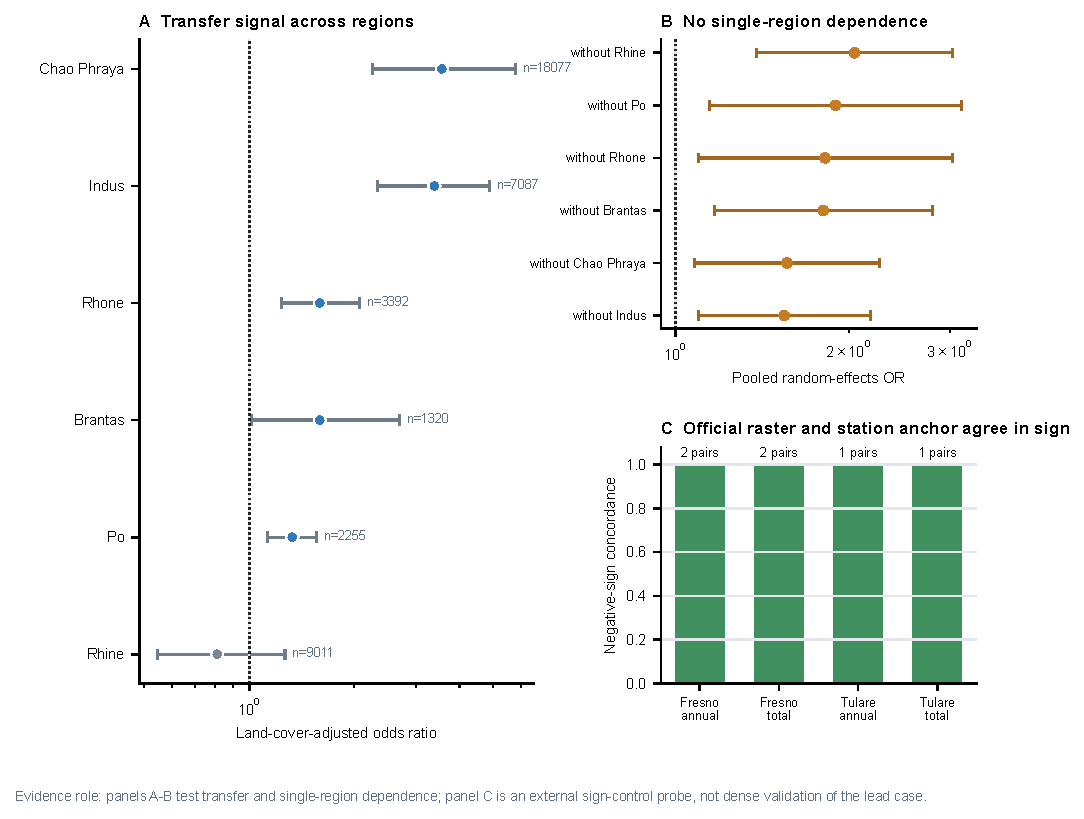
\includegraphics[width=0.98\linewidth]{ESIN_Supplementary_Figure_S3.pdf}
  \caption{Reviewer-risk experiments for transfer, single-region dependence and external sign control. Panel A reports land-cover-adjusted observability-bias odds ratios across six regions. Panel B reports leave-one-region-out random-effects estimates, showing that the pooled signal remains above unity when any single region, including the lead Chao Phraya case, is omitted. Panel C reports sign concordance between official DWR raster summaries and nearby NGL station anchors in the Central Valley positive-control setting. These checks strengthen transfer and external-control evidence but are not interpreted as dense validation of the lead hidden-exposure estimate.}
  \label{fig:S3}
\end{figure}

\section*{Supplementary Tables}

\begin{table}[htbp]
\centering
\caption{Evidence-role inventory for the ESIN submission package.}
\label{tab:S1}
\scriptsize
\setlength{\tabcolsep}{3pt}
\renewcommand{\arraystretch}{0.92}
\begin{tabular}{p{0.20\linewidth}p{0.20\linewidth}p{0.26\linewidth}p{0.23\linewidth}}
\toprule
Evidence layer & Role & Completed result or file status & Claim boundary \\
\midrule
Chao Phraya GHSL closure & Lead exposure closure & 3.77 M hidden people; 404.77 km$^2$ hidden built-up; native-pixel sensitivity gives 3.63 M people & Retained exposure, not confirmed affected population \\
Threshold surface & Robustness check & 120 combinations; 1.33--5.36 M people and 140.44--523.64 km$^2$ built-up & Sensitivity surface, not posterior interval \\
MAUP and shifted origins & Reporting-partition check & 3, 5, 10 and 20 cell blocks; hidden fractions preserved & Not exhaustive spatial-unit proof \\
Monte Carlo propagation & Scenario uncertainty & 5000 iterations; population p05/p50/p95 = 1.64/3.65/5.48 M & Scenario uncertainty, not product confidence \\
Placebo randomization & Falsification check & OR = 5.78 versus spatial-null mean 3.38; random masks gave larger exposure totals & Tests random artefacts, not deformation truth \\
Decision ranking & Operational check & At 2000 cells, overlap = 0.9365; added 572,297 hidden people and 10.83 km$^2$ built-up & Not cost-benefit or damage modelling \\
Po and Brantas & Transfer checks & Po OR = 2.60 (95\% CI 1.95--3.47); Brantas supports positive transfer & Not dense EGMS validation \\
Rhone and Rhine & Conditional/control checks & Rhone conditional; Rhine non-positive control/specification case & Proxy-level evidence \\
DWR/TRE--GHSL & External positive control & Tulare/Corcoran strong pixels contain 102,164 people and 18.81 km$^2$ built-up & Not Chao Phraya validation \\
Cyprus EGMS & Boundary/code-path control & 17,340 overlays; 65 strong points and 0.31\% population share at 5 mm yr$^{-1}$ & Near-zero tile, not strong benchmark \\
Po/Rhone EGMS hooks & Future benchmark & Payloads, runbook and closure code prepared & Not evidence until products are overlaid \\
\bottomrule
\end{tabular}
\end{table}

\begin{table}[htbp]
\centering
\caption{Major-revision risks addressed by added experiments.}
\label{tab:S2}
\scriptsize
\setlength{\tabcolsep}{3pt}
\renewcommand{\arraystretch}{0.92}
\begin{tabular}{p{0.22\linewidth}p{0.32\linewidth}p{0.34\linewidth}}
\toprule
Reviewer risk & Experiment or check & Remaining boundary \\
\midrule
Single-case dependence & Multi-region land-cover-adjusted forest plot and leave-one-region-out random-effects analysis & Supports transfer of the audit signal, not pooled global exposure \\
Threshold or partition artefact & Threshold surface, MAUP shifted-origin tests and native-pixel allocation & Shows persistence across tested choices, not universal invariance \\
Random hidden-mask explanation & Placebo randomization of strong labels and hidden masks & Falsifies random-placement alternatives, not deformation causality \\
Weak external evidence & DWR/GHSL positive control, DWR/NGL sign concordance and Cyprus EGMS near-zero boundary control & Bounds code-path and sign behavior, not dense Chao Phraya validation \\
Overclaiming hidden exposure & Evidence-role inventory and bounded-evidence protocol & Hidden exposure remains retained weak-observability exposure, not confirmed affected population \\
Reproducibility concern & Source-data inventory, runbooks, figure source data and release metadata & Credentialed EGMS extensions remain prepared hooks unless product access is available \\
\bottomrule
\end{tabular}
\end{table}

\section*{Supplementary Source Data}

The supplementary figures are generated from the MAUP sensitivity table, placebo randomization outputs, multi-region meta-closure tables and external-control summaries included in the submission package. The corresponding source files are:

\begin{itemize}
  \item \texttt{chao\_phraya\_maup\_sensitivity\_v1.csv}
  \item \texttt{chao\_phraya\_placebo\_randomization\_summary\_v1.csv}
  \item \texttt{chao\_phraya\_placebo\_randomization\_draws\_v1.csv}
  \item \texttt{multi\_region\_meta\_closure\_region\_table.csv}
  \item \texttt{multi\_region\_meta\_closure\_leave\_one\_out.csv}
  \item \texttt{dwr\_ngl\_station\_validation\_stats\_v1.csv}
  \item \texttt{ESIN\_Supplementary\_Figure\_S3\_source\_data.csv}
  \item \texttt{Q1\_STYLE\_EXPERIMENT\_STRENGTHENING\_20260719.csv}
  \item \texttt{external\_control\_synthesis\_v1.csv}
\end{itemize}

\end{document}
